

\ssn{Mathematical background}   \label{intfact}
Let $a,b$ be non-negative integers.  Then 
 \[
   I_{a,b} \stackrel{\text{def}}{=}  
   \int_0^1 x^a (1-x)^b \dd x = \frac{a! b!}{(a+b+1)!}. 
 \]
To establish this, first check with a trivial integration that $I_{0,b}= 1/(1+b)$. Then integrate by parts (differentiating the ``$x^a$'' term) to establish that 
 \[
     I_{a,b} = \frac{a}{b+1} I_{a-1,b+1}.
 \]
 Chasing through the consequences of this, we obtain the result. (Strictly, an induction proof would be appropriate.) 
\end{n}




\ssn{The Beta distribution}
Given that fact, we can define a family of random variables on $[0,1]$. We say that $X$ has a \emph{Beta distribution with parameters $\alpha, \beta \in \mathbb N$} if it has pdf
\[
    f_X(x) =   \frac{\Gamma(\alpha+\beta)}{\Gamma(\alpha) \Gamma(\beta)}  x^{\alpha-1}  (1-x)^{\beta -1}, \qquad x \in [0,1]. 
\]
We will concentrate on the case where $\alpha,\beta$ are positive integers but more generally, they can be positive real numbers. 
\end{n}

\ssn{A problem}
We will devote ourselves for a while to the following problem. Consider $n$ points independently uniformly distributed on $[0,1]$. What can I say about where the $k$-th largest point is?  So, for instance, the first non-trivial instance of the problem is to ask for the distribution of $\min(x_1,x_2)$ where $x_1, x_2$ are independently uniformly distributed on $[0,1]$. 
\end{n}


\ssn{Solving the problem}
Let us now solve the problem of the probable location of the k-th smallest point of $n$ points $x_1, \dots , x_n$ independently, uniformly distributed on $[0,1]$.  Let $f_{k,n}(x)$ be the pdf of its location and let $F_{k,n}(x)$ be the cumulative distribution function.  We will compute the latter and differentiate to obtain the pdf. 

Obtaining the cdf is the easy part: the $k$-th smallest of the points is less than or equal to $x$ precisely if at least $k$ of the $n$ points are less than $x$.  That is simply a binomial distribution with probability $p=x$ and so 
 \[
     F_{k,n}(x) = \sum_{j=k}^n \binom{n}j x^j (1-x)^{n-j}.
 \]
 Differentiating we obtain
 \begin{eqnarray*}
   f_{k,n}(x) &=& \frac{\dd}{\dd x} \sum_{j=k}^n \binom{n}j x^j (1-x)^{n-j}\\
   &=& \sum_{j=k}^n \left(
     j \binom{n}j x^{j-1}(1-x)^{n-j} - (n-j)\binom{n}j x^j (1-x)^{n-j-1}
   \right) \\
   &=& \sum_{j=k}^n 
     j \binom{n}j x^{j-1}(1-x)^{n-j} - 
     \sum_{j=k}^{n-1}  (n-j)\binom{n}{j} x^{j} (1-x)^{n-j-1}
 \end{eqnarray*}
where in that last step I split the sum in two and changed its upper limit to $j=n-1$ since when $j=n$ the factor $(n-j)$ makes it zero anyway. Continuing, substitute $j=j'-1$ in the second sum to obtain 
\begin{eqnarray*}
  f_{k,n}(x) &=& \sum_{j=k}^n 
     j \binom{n}j x^{j-1}(1-x)^{n-j} - 
     \sum_{j'=k+1}^{n}  (n-j'+1)\binom{n}{j'-1} x^{j'-1} (1-x)^{n-j'}
\end{eqnarray*}
Combining the coefficient of $x^{j-1}(1-x)^{n-j}$ in the two sums we have 
 \[
     j\binom{n}j - (n-j+1) \binom{n}{j-1} = \frac{n!}{(j-1)!(n-j)!} - 
     \frac{n!}{(j-1)!(n-j)!} = 0 
 \]
 except for the single case where $j=k$ and the term in the second sum does not exist. 

So  \[
    f_{k,n}(x) = \frac{n!}{(k-1)! (n-k)!} x^{k-1} (1-x)^{n-k}
 \]
which we recognise as a Beta distribution with parameters $\alpha=k$ and $\beta = n-k+1$. 
\end{n}

\begin{figure}[h] 
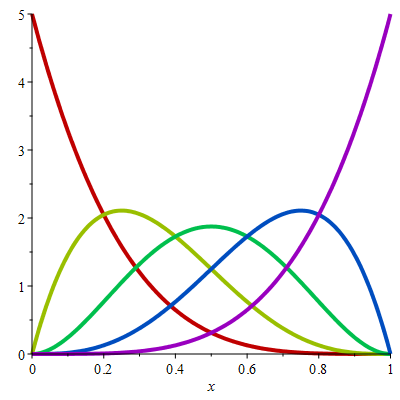
\includegraphics[width=0.45\textwidth]{images/beta5.png}\quad 
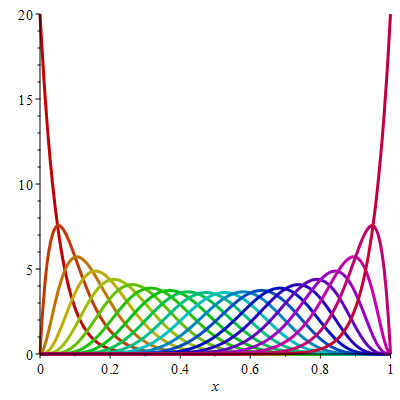
\includegraphics[width=0.45\textwidth]{images/beta20.png}
\caption{Pdf of position of $k$-th smallest of 5 (left) and 20 (right) independent, uniformly distributed numbers in $[0,1]$.  \label{kptpic}}
\end{figure}


\sse 
Compute the expected position of the $k$-th largest of $n$ independent, uniformly distributed numbers in $[0,1]$.  
\end{e}

\sss 
From the notes the pdf for the $k$th smallest of $n$ is 
\[
    f_{k,n}(x) = \frac{n!}{(k-1)! (n-k)!} x^{k-1} (1-x)^{n-k}. 
 \]
So its expected value is obtained by multiplying by $x$ and integrating: 
 \[
   \EE(X_{k,n}) = \int_0^1  \frac{n!}{(k-1)! (n-k)!} x^{k} (1-x)^{n-k}
   =  \frac{n!}{(k-1)! (n-k)!} \int_0^1   x^{k} (1-x)^{n-k}.
  \]
Using \S\ref{intfact} we evaluate the integral to be 
 \[
 \frac{n!}{(k-1)! (n-k)!} \, \frac{k! (n-k)!}{(n+1)!} = \frac{k}{n+1}.
 \]
\end{s}



\ssp 
Looking at the graphs in Figure~\ref{kptpic}, explain the following features, using mainly words rather than formulas. 
\begin{itemize}
\item Each picture is symmetric about the midpoint of the interval.
\item In the left-hand picture, the central blue-green graph is itself symmetric about the mid-point.
\item In both pictures, two of the graphs have non-zero values at one of the endpoints, but all the rest are zero at both end-points. 
\end{itemize}
\end{e}

\sss
\begin{itemize}
\item This is because the $k$-th smallest particle becomes the $k$-th largest particle if you reflect the interval in the mid-point. 
\item if there are an odd number $2k+1$ of particles, then the $k+1$-th particle reflects to itself under the symmetry just mentioned. 
\item The probability of having one particle in the interval $[0,\Delta t]$ is $n \Delta t$ as $\Delta t \map 0$.  So the corresponding distribution function approaches $n$ at the endpoints. But the probability of two points in such an interval is proportional to $(\Delta t)^2$ and so the distribution function must be zero at the end points. 
\end{itemize}
\end{s}

\ssp (Challenge)
This gives an alternative solution to the $k$-th smallest point problem. 

Let $f_{k,n}(x)$ be the pdf of its location. Then, in the limit as $\Delta x \map 0$ the probability of the $k$-th smallest point being in the interval $[x,x+\Delta x]$ is $f_{k,n}(x) \Delta x$. 

For that to happen, two things have to occur. Firstly, one of the $n$ points needs to be in that interval. (The possibility of more than one being in the interval can be neglected in the limit.) Secondly, given that one point is in that interval, $k-1$ of the remaining $n-1$ must be to the left of it and so in the interval $[0,x]$. 

Derive the solution from these considerations. 
\end{e}

